\documentclass[11pt,xcolor=table,aspectratio=169]{beamer}
\usetheme{CambridgeUS}
\usecolortheme{dolphin}

%\usepackage[utf8]{inputenc}
\usepackage[utf8]{inputenc}
\usepackage[lithuanian]{babel}
\usepackage[L7x]{fontenc}


\usepackage{amsmath}
\usepackage{amsfonts}
\usepackage{amssymb}
\usepackage{graphicx}

\usepackage{subcaption}
\usepackage{booktabs}
\usepackage{multirow} % for multirow tables
\setbeamertemplate{caption}[numbered] % for numbering captions
\usepackage{bm} %boldmath
\usepackage{eurosym}
\usepackage{float}
\usepackage{hyperref}
\hypersetup{
  colorlinks=true,
  linkcolor=black,
  filecolor=blue,   
  urlcolor=blue,
  citecolor=blue
}

\usepackage{booktabs}
\usepackage{hyperref}


\author{Irma Meškauskaitė, Valė Meilūnienė}
\title{Konvergencija}
%\setbeamercovered{transparent} 
\setbeamertemplate{navigation symbols}{} 
%\logo{} 
%\institute{} 
\date{\today} 
%\subject{} 

\graphicspath{{./figures/}}

\begin{document}

\begin{frame}
\titlepage
\end{frame}

%\begin{frame}
%\tableofcontents
%\end{frame}

\begin{frame}{Gyvenimo trukmė ES Šalyse}
\begin{itemize}
\item Lietuvoje vidutinė tikėtina gyvenimo trukmė siekia xx metų
\item ES vidurkis sieka xx metų
\begin{itemize}
\item Tralalala
\item Tralala
\end{itemize}
\item Mažiausia gyvenimo trukmė yra Ruminoje ir siekia xx metu
\item Ilgiausia ....
\end{itemize}
\end{frame}


\begin{frame}{Gyvenimo trukmė ES Šalyse}
\begin{figure}
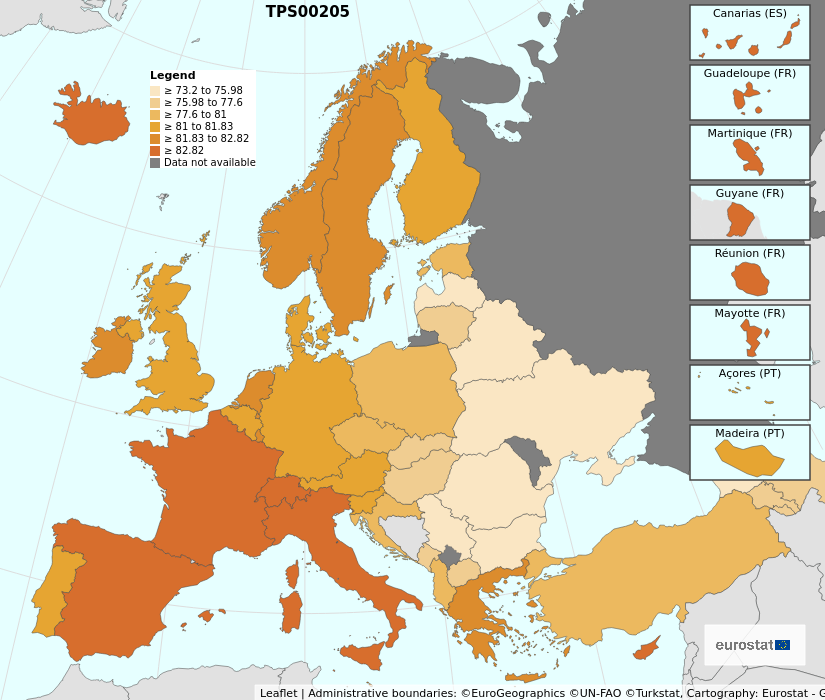
\includegraphics[scale=0.275]{TPS00205_MAP_CNTR_2020-11-26T12 10 12Z.png}
\end{figure}
\end{frame}


\begin{frame}{Gyvenimo trukmė ES Šalyse}
\begin{figure}
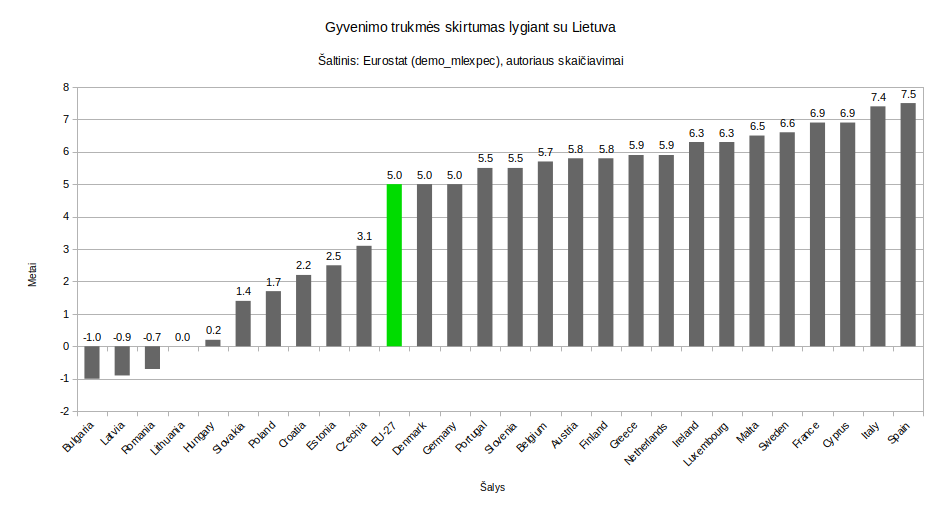
\includegraphics[scale=0.35]{bar_chart_eu_diff_lt.png}
\end{figure}
\end{frame}


\begin{frame}
% Please add the following required packages to your document preamble:
% \usepackage{booktabs}
\begin{table}[]
\begin{tabular}{@{}lll@{}}
\toprule
GEO/SEX   & vs\_LT & Total \\ \midrule
Bulgaria  & -1     & 75    \\
Latvia    & -0.9   & 75.1  \\
Romania   & -0.7   & 75.3  \\
Lithuania & 0      & 76    \\
Hungary   & 0.2    & 76.2  \\
Slovakia  & 1.4    & 77.4  \\ \bottomrule
\end{tabular}
\end{table}
\end{frame}


\end{document}